\documentclass[a4paper,12pt]{article}
\usepackage{fullpage}
\usepackage{amsmath}
\usepackage{graphicx}
\usepackage{subfig}
\usepackage{setspace}
\usepackage{bm}
\usepackage{etoolbox}
\doublespace

\setlength{\abovedisplayskip}{0pt}
\setlength{\belowdisplayskip}{0pt}
\setlength{\abovedisplayshortskip}{0pt}
\setlength{\belowdisplayshortskip}{0pt}

\BeforeBeginEnvironment{equation}{\begin{singlespace}}
\AfterEndEnvironment{equation}{\end{singlespace}\noindent\ignorespaces}
\BeforeBeginEnvironment{align}{\begin{singlespace}}
\AfterEndEnvironment{align}{\end{singlespace}\noindent\ignorespaces}

\renewcommand{\vec}[1]{\boldsymbol{\mathbf{#1}}}

\setlength{\parindent}{0pt} 

\begin{document}

\textbf{\large Berry Phase} \\

\textbf{Adiabatic approximation}: Hamiltonian depends on parameters $\vec{R}$.  If $\vec{R}$ changes very slowly, and you start in the $n$th eigenstate, you will stay in the $n$th eigenstate (instead of transitioning to an $m$th eigenstate - see Griffiths QM for proof).  For example, the infinite square well with $L$ changing to $2L$ and then back to $L$:

\begin{figure}[h!]
\centering
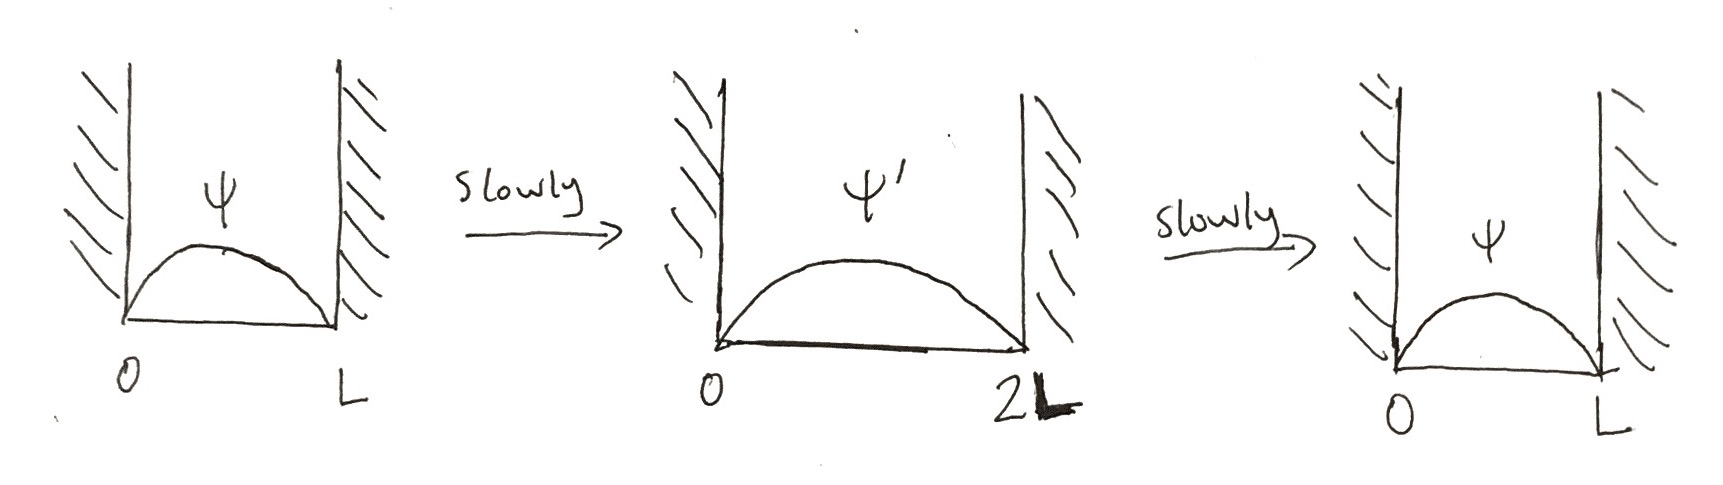
\includegraphics[width=150mm,keepaspectratio=true]{infinitewell.jpg}
\end{figure}

So if $\vec{R}$ (or $L$ in this example) goes back to it's original value, you will return to the original state.  However (in non-1D examples), the phase might be different!
\\ \\
\textbf{Classical Example}: Carry an arrow that always points south from the north pole of a sphere to the equator, then along the equator, then back to the north pole.  The arrow will be rotated compared to its original direction by an angle $\gamma$ that depends on how far the arrow was carried along the equator.  This angle $\gamma = \text{Arc Length}/\text{Radius of Sphere}$ is called the Berry phase, and it's caused by the curvature of the sphere.
\\
\begin{figure}[h!]
\centering
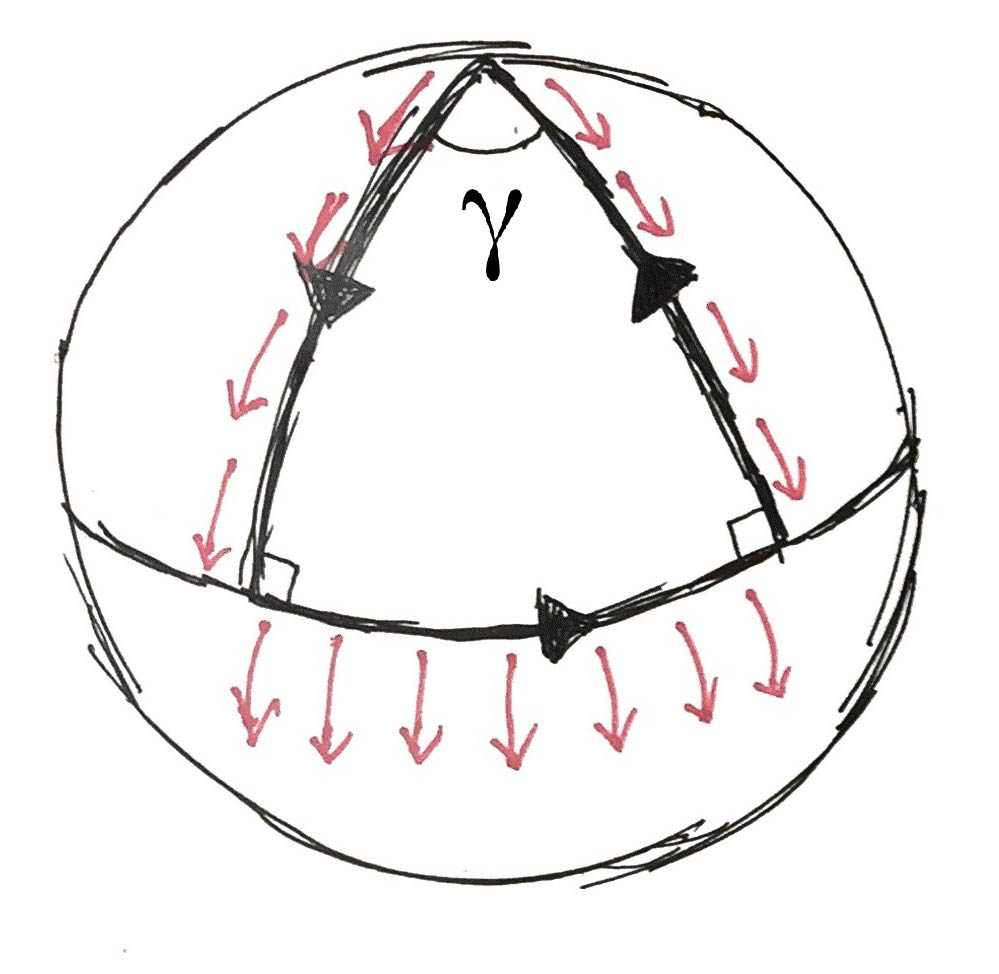
\includegraphics[width=50mm,keepaspectratio=true]{geometric.jpg}
\end{figure}

In the arrow on a sphere example, we are moving a vector around a ``bundle" of vector spaces (each point on the sphere looks like a flat plane, so a sphere is really an infinite collection of 2D vector spaces parameterized by coordinates $\theta$ and $\phi$).
\\ \\
In direct analogy, we can imagine moving a quantum vector around a bundle of Hilbert spaces parameterized by $\vec{R}$ (which is not always a position coordinate).  Like the arrow on a sphere, the quantum vector will also develop a Berry phase when it returns to its initial state.  Lets calculate the Berry phase for a quantum state:
\begin{equation}
H(\vec{R}) | n(\vec{R}) \rangle = E(\vec{R}) | n(\vec{R}) \rangle
\end{equation}

\begin{figure}[h!]
\centering
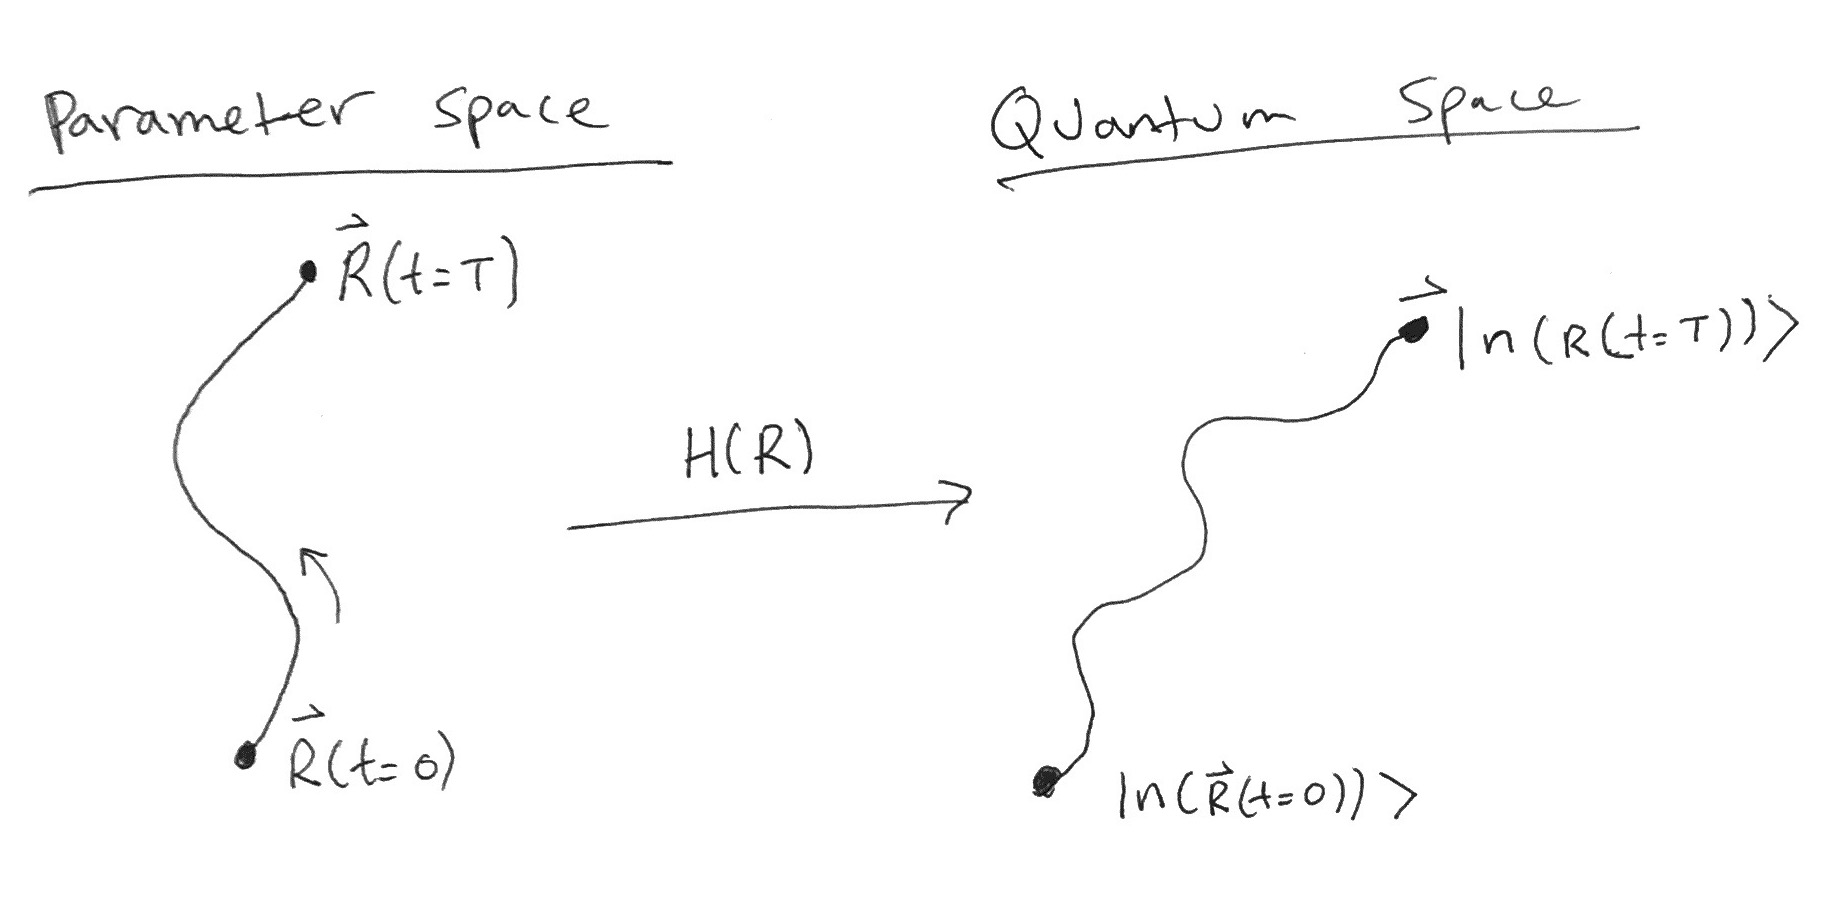
\includegraphics[width=150mm,keepaspectratio=true]{param.jpg}
\end{figure}

Here $\vec{R}=\vec{R}(t)$ is a set of parameters that vary slowly with time from initial time $t=0$ to final time $t=T$.

We can write the time dependent wavefunction as a phase times the eigenstate
\begin{equation}
| \Psi(\vec{R},t) \rangle = e^{i\theta(t)} | n(\vec{R}) \rangle
\end{equation}

and plug into the Schrodinger Equation $H(\vec{R}) | \Psi(\vec{R},t) \rangle = i\hbar \frac{\partial}{\partial t} | \Psi(\vec{R},t) \rangle$ to get
\begin{equation}
e^{i\theta(t)} E(\vec{R}) | n(\vec{R}) \rangle = -\hbar \frac{d\theta(t)}{dt} e^{i\theta(t)} | n(\vec{R}) \rangle + i\hbar e^{i\theta(t)} \frac{d}{dt} | n(\vec{R}) \rangle
\end{equation}
and multiply both sides by $\langle n(\vec{R}) |$
\begin{equation}
\frac{d\theta}{dt}=-\frac{E(\vec{R})}{\hbar}+i \langle n(\vec{R}) | \frac{d}{dt} | n(\vec{R}) \rangle
\end{equation}
Integrate it.
\begin{equation}
\theta(T)=-\frac{1}{\hbar} \int_0^T E(\vec{R}(t))dt+i \int_0^T \langle n(\vec{R}) | \frac{d}{dt} | n(\vec{R}) \rangle dt
\end{equation}
The first term is the dynamic phase caused the regular time evolution of an energy eigenstate. Here, it is $e^{-\frac{i}{\hbar} \int_0^T E(\vec{R}(t))dt}$ instead of $e^{-iET/\hbar}$ because energy is not constant with time.  We pump energy in and out of the system by slowing varying parameters $\vec{R}$ as a function of time.
\\ \\
The second term
\begin{equation}
\gamma=i \int_0^T \langle n(\vec{R}) | \frac{d}{dt} | n(\vec{R}) \rangle dt=i \int_C \langle n(\vec{R}) | \nabla_{\vec{R}} | n(\vec{R}) \rangle \cdot d\vec{R}
\end{equation}
is the Berry phase (also called geometric phase).  It's completely analogous to the classical arrow moving around on a sphere.
\\ \\
Is the Berry phase actually a phase?  To be a phase, it needs to be a real number.  Here is a proof:
\begin{equation}
\frac{d}{dt} \langle n(\vec{R}) | n(\vec{R}) \rangle = \frac{d}{dt}(1)=0
\end{equation}
because $| n(\vec{R}) \rangle$ is normalized.  This implies
\setlength{\jot}{15pt}
\begin{eqnarray}
\left( \frac{d}{dt} \langle n(\vec{R}) | \right) | n(\vec{R}) \rangle + \langle n(\vec{R}) | \left( \frac{d}{dt} | n(\vec{R}) \rangle \right) = 0 \\
\left[ \langle n(\vec{R}) | \frac{d}{dt} | n(\vec{R}) \rangle \right]^* = - \left[ \langle n(\vec{R}) | \frac{d}{dt} | n(\vec{R}) \rangle \right]
\end{eqnarray}
So $\langle n(\vec{R}) | \frac{d}{dt} | n(\vec{R}) \rangle$ is purely imaginary, and the Berry phase is real.
\\ \\
Some more terminology:
\begin{equation}
\vec{A}(\vec{R})=i \langle n(\vec{R}) | \nabla_{\vec{R}} | n(\vec{R}) \rangle
\end{equation}
is called the Berry connection.  We give it the symbol $\vec{A}$ because it shares many properties with the magnetic vector potential.  In particular, if $\vec{R} = (R_x, R_y, R_z)$, then we can take the curl of $\vec{A}$ to get
\begin{equation}
\vec{\Omega}(\vec{R}) = \nabla_{\vec{R}} \times \vec{A}(\vec{R})
\end{equation}
is called the Berry curvature.
\\ \\
If $\vec{R}(t=0) = \vec{R}(t=T)$, we can apply Stoke's Theorem
\begin{equation}
\gamma = \int \vec{\Omega}(\vec{R}) \cdot d\vec{S}
\end{equation}
What happens if we change the phase convention of the eigenstates of $H(\vec{R})$?  Suppose we multiplied $| n(\vec{R}) \rangle$ by a phase factor $e^{-i\chi(\vec{R})}$, where $\chi(\vec{R})$ is some arbitrary function:
\begin{equation}
| n(\vec{R}) \rangle \rightarrow e^{-i\chi(\vec{R})} | n(\vec{R}) \rangle
\end{equation}
Then
\begin{eqnarray}
\vec{A}(\vec{R}) &\rightarrow& i \left( \langle n(\vec{R}) | e^{i\chi(\vec{R})} \right) \nabla_{\vec{R}} \left( e^{-i\chi(\vec{R})} | n(\vec{R}) \rangle \right) \\
\vec{A}(\vec{R}) &\rightarrow& i \left( \langle n(\vec{R}) | e^{i\chi(\vec{R})} \right) \left( e^{-i\chi(\vec{R})} \nabla_{\vec{R}} | n(\vec{R}) \rangle -ie^{-i\chi(\vec{R})} \left( \nabla_{\vec{R}} \chi(\vec{R}) \right) | n(\vec{R}) \rangle \right) \\
\vec{A}(\vec{R}) &\rightarrow& \vec{A}(\vec{R}) + \nabla_{\vec{R}} \chi(\vec{R})
\end{eqnarray}
and because $\nabla_{\vec{R}} \times \nabla_{\vec{R}} \chi(\vec{R}) = 0$, $\vec{\Omega(\vec{R})}$ and therefore the Berry phase $\gamma$ does not change.  This means that the Berry phase is not arbitrary and is physically measurable.  Also, note that this looks exactly like the gauge transformation from electromagnetism. \\
Side note: In fact, it can be shown that the Berry phase produces a ``Lorentz force" $\frac{d\vec{R}}{dt} \times \vec{\Omega}$ in the classical equations of motion.
\\ \\
\textbf{Example Problem: Spin 1/2 in a Rotating Magnetic Field} \\
A spin in a magnetic field is described by the Hamiltonian
\begin{equation}
H = \vec{\mu} \cdot\vec{B} = \mu_0 \sigma \cdot \vec{B}
\end{equation}
We can write $\vec{B}$ in spherical coordinates: $\vec{B} = |\vec{B}| (\sin\theta \cos\phi, \sin\theta \sin\phi, \cos\theta)$ \\
Then
\begin{equation}
H = \mu_0 |\vec{B}| \left(
\begin{matrix}
\cos{\theta} & \sin{\theta} e^{-i \phi}  \\
\sin{\theta} e^{i \phi} & -\cos{\theta}
\end{matrix}
\right)
\end{equation}
The eigenvector where spin points in the direction of $\vec{B}$ is given by
\begin{equation}
\chi_+ = \left(
\begin{matrix}
\cos{\frac{\theta}{2}} \\
e^{i \phi} \sin{\frac{\theta}{2}}
\end{matrix}
\right)
\end{equation}
Griffiths QM calculates the Berry phase for $\chi_+$ the long way using
\begin{equation}
\nabla_{(B_x,B_y,B_z)}=\frac{\partial}{\partial r} \hat{r} + \frac{1}{r} \frac{\partial}{\partial \theta} \hat{\theta} + \frac{1}{r \sin \theta} \frac{\partial}{\partial \phi} \hat{\phi}
\end{equation}
but there's a faster way to do this problem: Just pretend $\theta$ and $\phi$ are Cartesian coordinates.  The final answer must be the same in the end because all of the formalism developed so far is for generic parameters $\vec{R}(t)$, which can be anything.
\begin{equation}
\nabla_{(\theta, \phi)}=\frac{\partial}{\partial \theta} \hat{\theta} + \frac{\partial}{\partial \phi} \hat{\phi}
\end{equation}
Then
\begin{eqnarray}
A_{\theta} &=& i \langle \chi_+ | \frac{\partial}{\partial \theta} | \chi_+ \rangle = i \left(
\begin{matrix}
\cos{\frac{\theta}{2}} & e^{-i\phi} \sin{\frac{\theta}{2}}
\end{matrix}
\right)
\frac{\partial}{\partial \theta} \left(
\begin{matrix}
\cos{\frac{\theta}{2}} \\
e^{i\phi} \sin{\frac{\theta}{2}}
\end{matrix}
\right) = 0
\\
A_{\phi} &=& i \langle \chi_+ | \frac{\partial}{\partial \phi} | \chi_+ \rangle = i \left(
\begin{matrix}
\cos{\frac{\theta}{2}} & e^{-i\phi} \sin{\frac{\theta}{2}}
\end{matrix}
\right)
\frac{\partial}{\partial \phi} \left(
\begin{matrix}
\cos{\frac{\theta}{2}} \\
e^{i\phi} \sin{\frac{\theta}{2}}
\end{matrix}
\right) = -\sin^2 \frac{\theta}{2}
\end{eqnarray}
Then the Berry curvature is the ``curl" of $\vec{A}$:
\begin{equation}
\Omega = \nabla_{(\theta,\phi)} \times \vec{A} = \partial_\theta A_\phi - \partial_\phi A_\theta = -\frac{1}{2} \sin \theta
\end{equation}
And the Berry phase is
\begin{equation}
\gamma = \int \Omega d\theta d\phi = -\frac{1}{2} \int \sin \theta d\theta d\phi
\end{equation}
But $\sin \theta d\theta d\phi$ is just the differential solid angle, so $\gamma = -\frac{1}{2} \left( \text{Solid Angle} \right)$.  If $\vec{B}(t) = |\vec{B}| (\cos \omega t, \sin \omega t, 0)$ rotates in the x-y plane, then the solid angle is $2\pi$ (half a sphere), so $\gamma = -\pi$.  This is a real measurable effect!  You can use this to get destructive interference of an electron wave. \\
The Berry phase for the opposite spin orientation $\chi_-$ is $\gamma = +\frac{1}{2} \left( \text{Solid Angle} \right)$.  It is a general property that the sum of the Berry phase over all states is zero.  Here is a proof:
\begin{eqnarray}
\vec{\Omega}(\vec{R}) &=& i \nabla_{\vec{R}} \times \langle n(\vec{R}) | \nabla_{\vec{R}} | n(\vec{R}) \rangle = -\text{Im} \left( \nabla_{\vec{R}} \times \langle n(\vec{R}) | \nabla_{\vec{R}} | n(\vec{R}) \rangle \right) \\
&=& -\text{Im} \left( \left[ \nabla_{\vec{R}} \langle n(\vec{R}) | \right] \times \left[ \nabla_{\vec{R}} | n(\vec{R}) \rangle \right] + \langle n(\vec{R}) | \nabla_{\vec{R}} \times \nabla_{\vec{R}} | n(\vec{R}) \rangle \right)
\end{eqnarray}
The second term on the right is zero because it's a curl of a gradient.  We can insert a complete set of states $1 = \sum_m | m(\vec{R}) \rangle \langle m(\vec{R}) |$.
\begin{eqnarray}
\vec{\Omega}(\vec{R}) &=& -\text{Im} \sum_m \left[ \nabla_{\vec{R}} \langle n(\vec{R}) | \right] | m(\vec{R}) \rangle \times \langle m(\vec{R}) | \nabla_{\vec{R}} | n(\vec{R}) \rangle \\
&=& -\text{Im} \sum_{m \ne n} \left[ \langle m(\vec{R}) | \nabla_{\vec{R}} | n(\vec{R}) \rangle \right]^* \times \langle m(\vec{R}) | \nabla_{\vec{R}} | n(\vec{R}) \rangle
\end{eqnarray}
where we dropped the $m = n$ term because $\langle n(\vec{R}) | \nabla_{\vec{R}} | n(\vec{R}) \rangle$ is purely imaginary, and so $\left[ \langle n(\vec{R}) | \nabla_{\vec{R}} | n(\vec{R}) \rangle \right]^* \times \langle n(\vec{R}) | \nabla_{\vec{R}} | n(\vec{R}) \rangle$ is real. Lets consider the quantity $\langle m(\vec{R}) | \nabla_{\vec{R}} \left(H | n(\vec{R}) \rangle \right)$:
\begin{eqnarray}
\langle m(\vec{R}) | \nabla_{\vec{R}} \left(H | n(\vec{R}) \rangle \right) &=& \langle m(\vec{R}) | \left( \nabla_{\vec{R}} H \right) | n(\vec{R}) \rangle + \langle m(\vec{R}) | \nabla_{\vec{R}} H | n(\vec{R}) \rangle \\
E_n(\vec{R}) \langle m(\vec{R}) | \nabla_{\vec{R}} | n(\vec{R}) \rangle &=& \langle m(\vec{R}) | \left( \nabla_{\vec{R}} H \right) | n(\vec{R}) \rangle + E_m(\vec{R}) \langle m(\vec{R}) | \nabla_{\vec{R}} | n(\vec{R}) \rangle
\end{eqnarray}
For the non-degenerate energy levels,
\begin{equation}
\langle m(\vec{R}) | \nabla_{\vec{R}} | n(\vec{R}) \rangle = \frac{\langle m(\vec{R}) | \left( \nabla_{\vec{R}} H \right) | n(\vec{R}) \rangle}{E_n(\vec{R})-E_m(\vec{R})}
\end{equation}
Finally,
\begin{equation}\label{eq:curvature}
\vec{\Omega}_n(\vec{R}) = -\text{Im} \sum_{m \ne n}{\frac{\langle n(\vec{R}) | (\nabla_{\vec{R}} H) | m(\vec{R}) \rangle \times \langle m(\vec{R}) | (\nabla_{\vec{R}} H) | n(\vec{R}) \rangle}{(E_m(\vec{R})-E_n(\vec{R}))^2}}
\end{equation}
It can be seen that the sum over all states $\sum_n \vec{\Omega}_n(\vec{R}) = 0$ because each term $\langle n(\vec{R}) | (\nabla_{\vec{R}} H) | m(\vec{R}) \rangle \times \langle m(\vec{R}) | (\nabla_{\vec{R}} H) | n(\vec{R}) \rangle$ can be paired with an opposite term where $n$ and $m$ are switched.
\\ \\
\textbf{Example: Forbidden Intravalley Backscattering in Graphene} \\
An amazing property graphene (and topological insulators) is that electrons in graphene are never reflected backwards $180^{\circ}$ by electric potentials even when the potential energy is bigger than the kinetic energy.  This can be explained by the Berry phase.
\begin{figure}[h!]
\centering
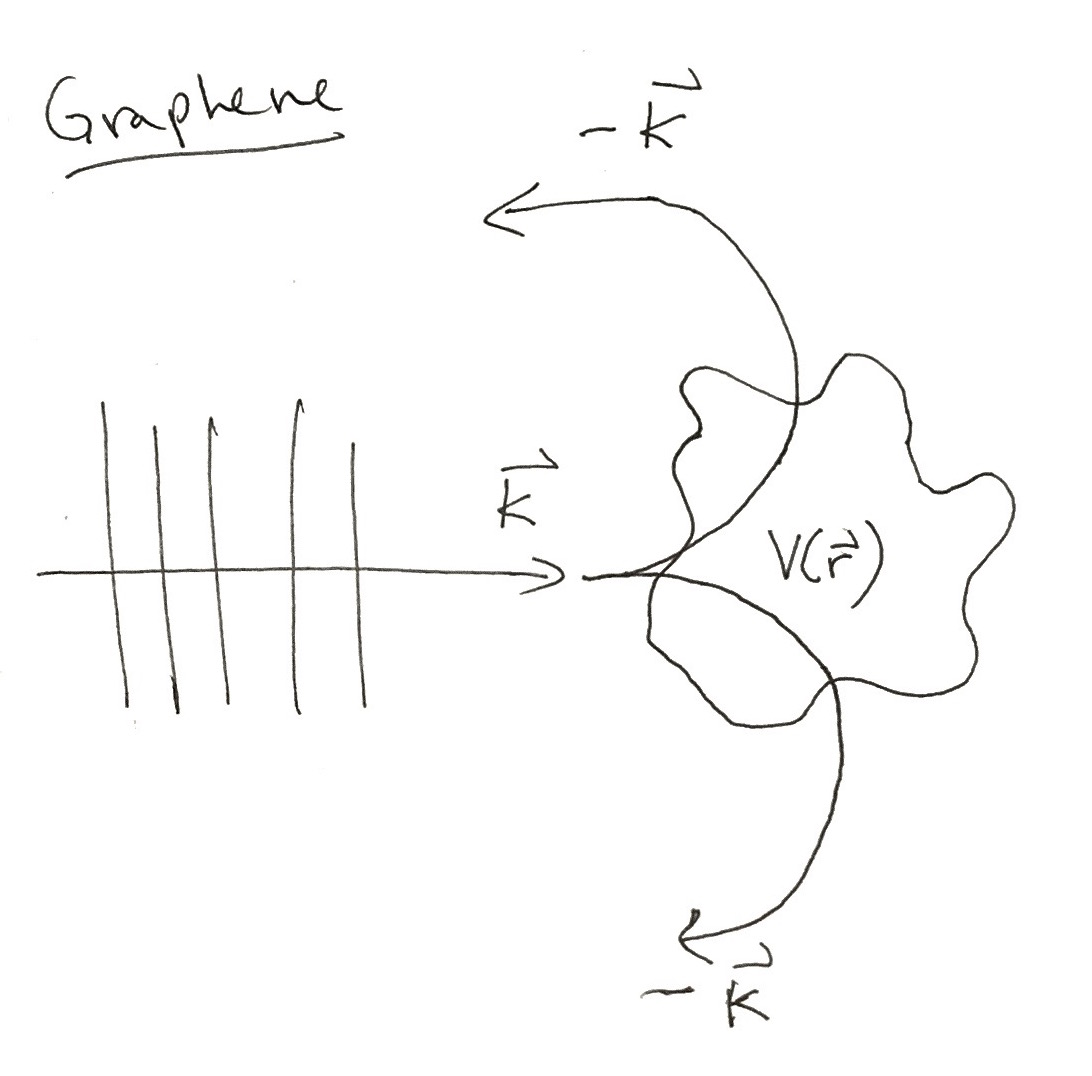
\includegraphics[width=100mm,keepaspectratio=true]{backscatter.jpg}
\end{figure}

Electrons in graphene behave like massless particles with spin. Then Hamiltonian is
\begin{equation}
H=\vec{\sigma} \cdot \vec{p} v = \hbar v \vec{\sigma} \cdot \vec{k}
\end{equation}
This looks exactly like the Hamiltonian for the spin in a magnetic field, $H = \mu_0 \sigma \cdot \vec{B}$, except with momentum $\vec{k}$ replacing magnetic field $\vec{B}$.  Then the Berry phase for $\vec{k}$ going around in a circle is $\pi$, and the Berry phase of going halfway around a circle (from $\vec{k}$ to $-\vec{k}$) is $\pi/2$.
\begin{figure}[h!]
\centering
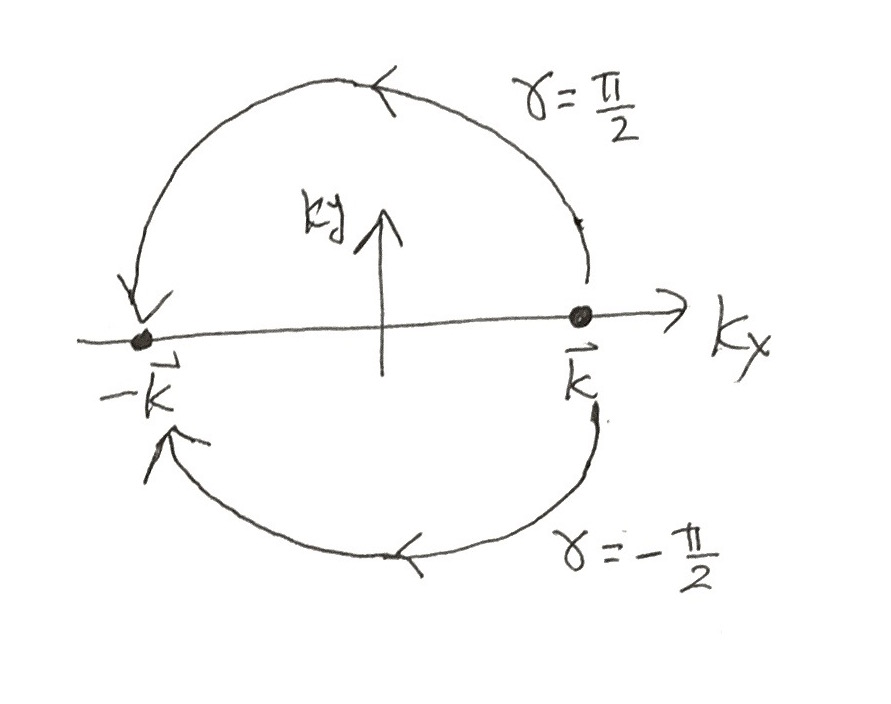
\includegraphics[width=100mm,keepaspectratio=true]{kspace.jpg}
\end{figure}

Every path from $\vec{k}$ to $-\vec{k}$ has a corresponding path that has opposite Berry phase (i.e. if one has $\gamma=\pi/2$, the other has $\gamma=-\pi/2$.  Then the reflected wave is a superposition of the two:
\begin{equation}
e^{i\pi/2}\psi(-\vec{k})+e^{-i\pi/2}\psi(-\vec{k}) = \left( 2 \cos \frac{\pi}{2} \right) \psi(-\vec{k}) = 0
\end{equation}
So there is destructive interference, and graphene electrons cannot be reflected $180^{\circ}$ by electric potentials.
\\ \\
\textbf{The Aharonov-Bohm Effect} \\
Imagine a solenoid with magnetic field $\vec{B}$ inside it.  There's no magnetic field outside the solenoid.  There's a particle in a box (with walls described by a potential $V(\vec{r}-\vec{R})$) outside the solenoid with wavefunction $\psi(\vec{r}-\vec{R})$. Let $\vec{A}(\vec{r})$ be the magnetic vector potential (not the Berry connection - confusingly, they share the same symbol). \\
The Hamiltonian is then
\begin{equation}
H=\frac{1}{2m} \left[ -i \hbar \nabla_{\vec{r}} - q \vec{A}(\vec{r}) \right]^2 + V(\vec{r}-\vec{R})
\end{equation}
\begin{figure}[h!]
\centering
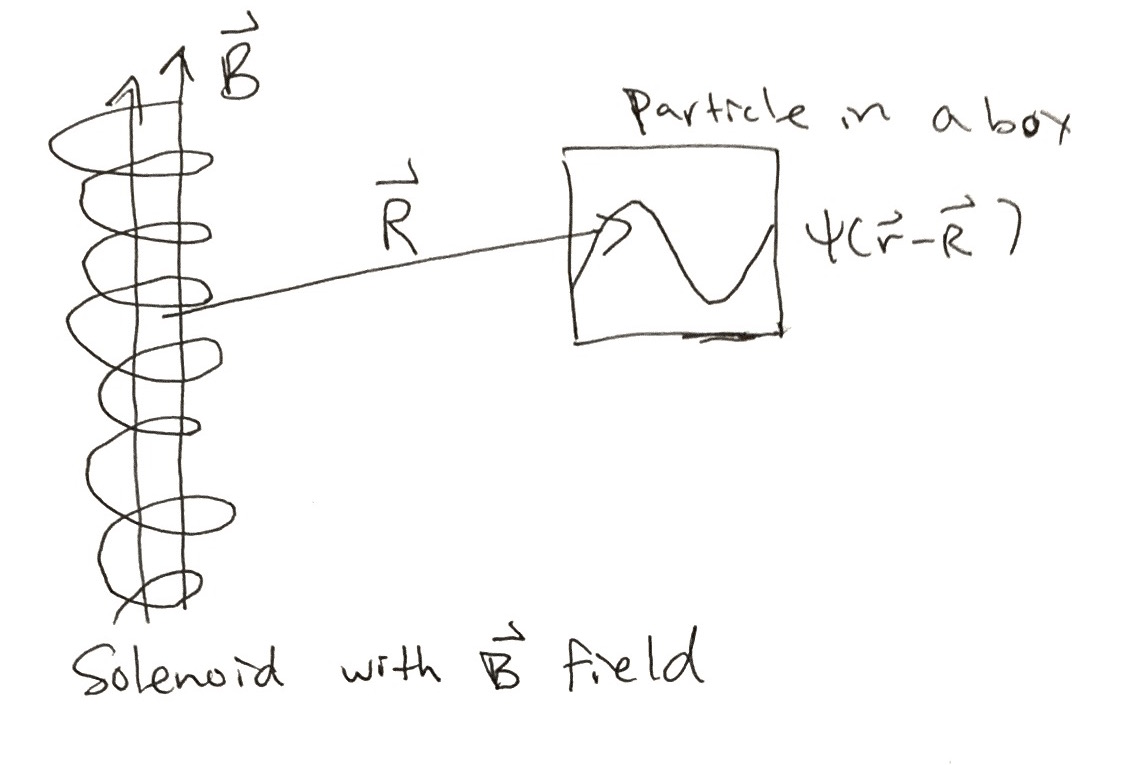
\includegraphics[width=150mm,keepaspectratio=true]{solenoid.jpg}
\end{figure}

If $\psi$ is a solution with $\vec{A} = 0$, then $\psi'=e^{i\frac{q}{\hbar} \int_R^r \vec{A}(\vec{r'}) \cdot d\vec{r'}}\psi(\vec{r}-\vec{R})$ is a solution for $\vec{A} \ne 0$.  Then, if the box is moved in a circle around the the solenoid, the Berry phase is
\begin{equation}
\gamma = i \oint \langle \psi' | \nabla_{\vec{R}} | \psi' \rangle \cdot d\vec{R}
\end{equation}
Just compute it.
\begin{eqnarray}
\nabla_{\vec{R}} \psi' &=& e^{i\frac{q}{\hbar} \int_R^r \vec{A}(\vec{r'}) \cdot d\vec{r'}} \left[ -i \frac{q}{\hbar} \vec{A}(\vec{R}) + \nabla_{\vec{R}} \right] \psi(\vec{r}-\vec{R}) \\
\langle \psi' | \nabla_{\vec{R}} | \psi' \rangle &=& -i \frac{q}{\hbar} \vec{A}(\vec{R}) + \int \psi(\vec{r}-\vec{R}) \nabla_{\vec{R}} \psi(\vec{r}-\vec{R}) d^3\vec{r}
\end{eqnarray}
The second term on the right is a momentum integral (because $\nabla_{\vec{R}} = -\nabla_{\vec{r}}$ when acting on $\psi(\vec{r}-\vec{R})$), so it is zero for the particle in the box.
\begin{equation}
i \langle \psi' | \nabla_{\vec{R}} | \psi' \rangle = \frac{q}{\hbar} \vec{A}(\vec{R})
\end{equation}
So it turns out that the Berry connection and magnetic vector potential are actually the same in this example.  The Berry phase is then
\begin{equation}
\gamma = \frac{q}{\hbar} \oint \vec{A}(\vec{R}) \cdot d\vec{R} = \frac{q}{\hbar} \int \vec{B} \cdot d\vec{S} = \frac{q}{\hbar} \left( \text{Magnetic Flux} \right)
\end{equation}
where we used Stokes's Theorem and the fact that $\vec{B} = \nabla \times \vec{A}$. \\
So even though the particle in the box never feels a Lorentz force (because $\vec{B} = 0$ everywhere outside the solenoid), the particle somehow knows that it circled around a magnetic field.
\\ \\
\textbf{Example: Electric Polarization} \\
The electric polarization of a solid is $\vec{P} = \sum e \vec{r}$.

\begin{figure}[h!]
\centering
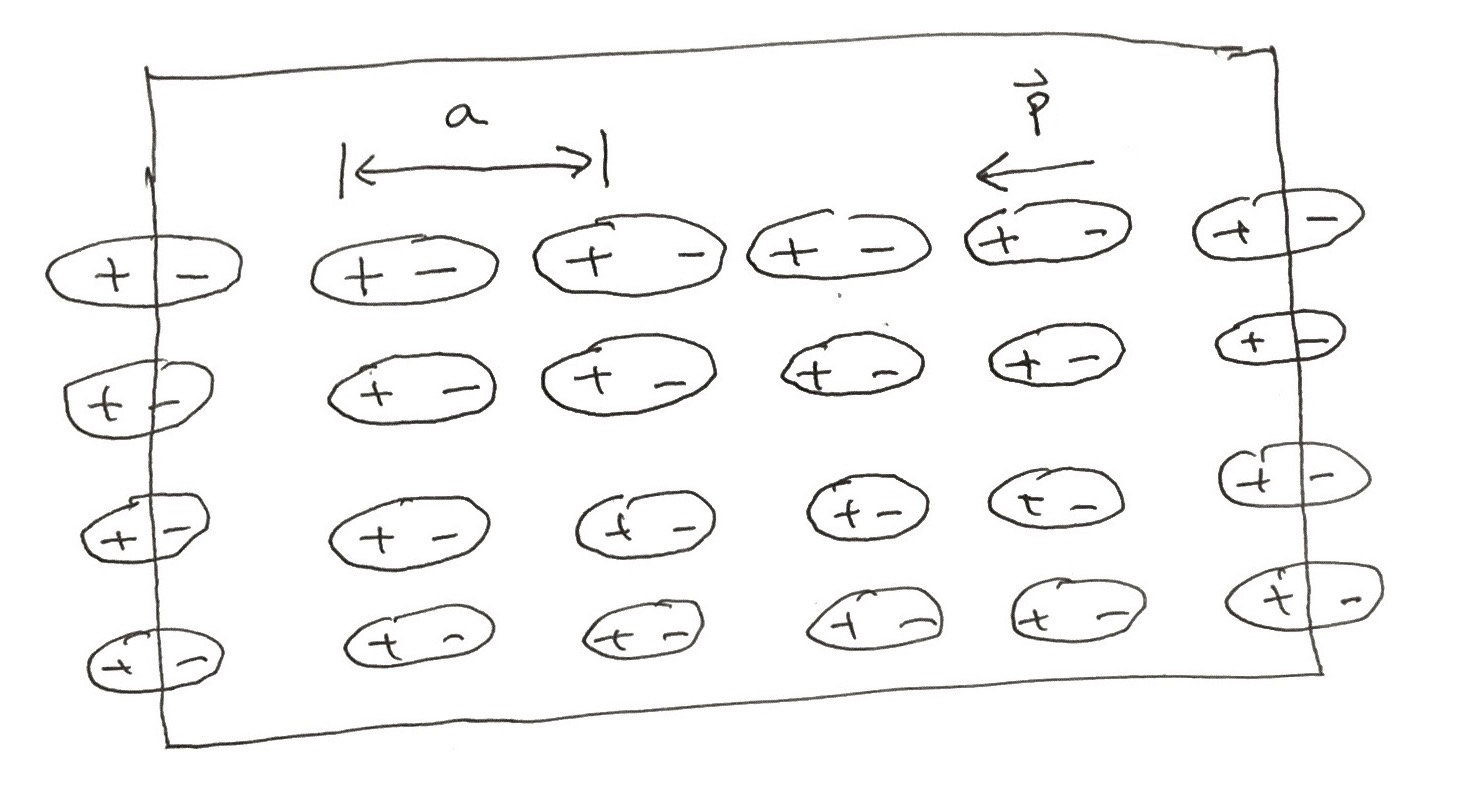
\includegraphics[width=100mm,keepaspectratio=true]{polarization.jpg}
\end{figure}

After some math using perturbation theory,
\begin{equation}
\vec{P} = e \int \frac{d^3\vec{k}}{(2\pi)^3} \langle u_{\vec{k}} | i \nabla_{\vec{k}} | u_{\vec{k}} \rangle
\end{equation}
where $u_{\vec{k}}(\vec{r}) = e^{-i\vec{k} \cdot \vec{r}} \psi_{\vec{k}}(\vec{r})$.  Intuitively (although not rigorously), this equation is true because $\vec{r} = i \hbar \nabla_{\vec{k}} $.  You can see that the polarization is an integral of the Berry connection.  Since electric polarization causes a surface charge at the interface of the dielectric, we see that somehow the Berry phase of wavefunctions in the bulk of a solid is related to physics at the boundary.  This is a very general principle.

\end{document}